\begin{multicols}{3}
\noindent \lettrine[lraise=0.2, nindent=0em, slope=-.5em]{Г}{имназия} "Гьоте" е 
една от гимназиите, основани преди 55 години в България, за да могат  учениците  
наред с общообразователните дисциплини да получават специализирано образование 
по езици. Училището, заедно с гимназия "Гълъбов "в София са единствени със 
самостоятелно преподаване на немски език.
В началото са четири класа по 20 ученици, като училището се помещава в сегашната 
сграда на гимназия „Г. С. Раковски” в Бургас. Първият директор на гимназия 
„Вилхелм Пик” е г-н Борис Баев. През 1965г. завършват гимназията първите 
единадесетокласници. Между 1967-1970г. директор на училището е г-н Христо 
Георгиев, а след това г-н Никола Владимиров. 1971г. училището се премества в 
сегашната си сграда. През 1981г. новият директор на гимназията е г-жа Пенка 
Мамарова, а през 1983г паралелките стават пет. Възпитаниците на гимназията се 
разпределят в шест паралелки през 1990г. и през същата година училището се 
преименува в гимназия „Гьоте”. 

\vspace{-5cm}

\begin{window}[2,r, 
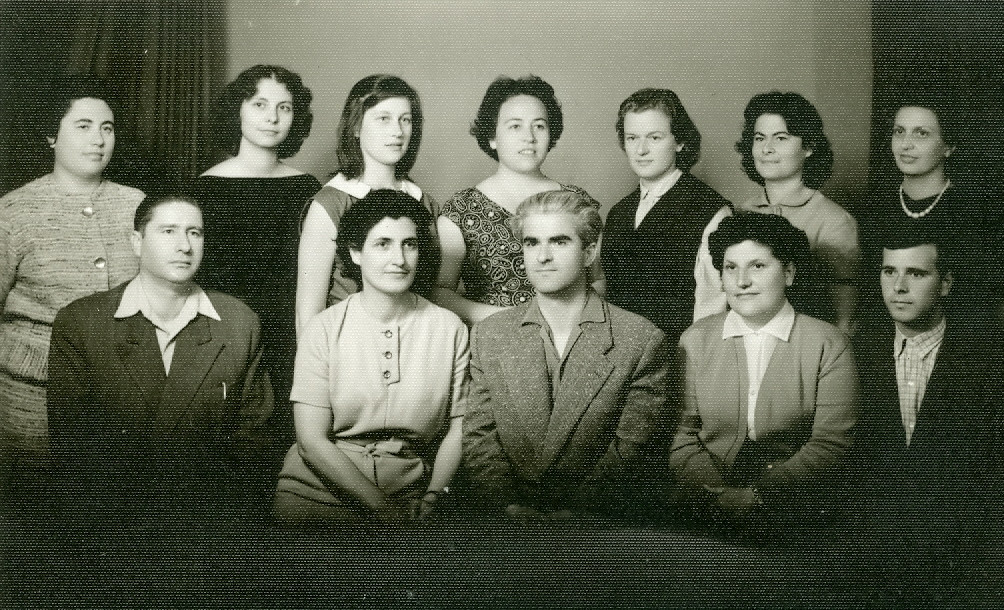
\includegraphics[width=4.4in]{./erste/1.jpg},\centerline{Първите учители}] 
\end{window}
През 1985г. гимназията е удостоена с орден „Кирил и Методий“, а от 1994 г.  е 
първото училище в цяла Източна Европа със сертификат за 
езикова диплома (КМК ІІ). От 1995г. училището е център за провеждане на изпити 
за България. Сертификатът за владеене на езика дава възможност на завършилите да 
постъпват в университети в Германия без приемни изпити. 
Носители на този документ са много младежи и девойки, голяма част от които в 
настоящия момент са студенти в европейски университети.
От 1996г. училището разполага с модерна компютърна зала,\\[0.1cm]  \\[7.55cm] включена и в Интернет.
Изграденият с помощта на спонсори от гр. Дюселдорф информационен 
център по немски език, разполага с много и разнообразна справочна и художествена 
литература, технически средства и връзка с Интернет. 
% \columnbreak
 От 1998г. гимназия “Гьоте” е включена в европейския проект 
“Коменски” (Comenius-Project) и работи успешно със своите партньори от Румъния, 
Полша, Швеция, Англия, Франция, Италия, Шотландия, Германия и Португалия. 
В гимназията се обучават около 800 ученици за 5 учебни години.  В 9-ти клас 
предметите биология и химия, а в 10-ти история и география,  се преподават  на 
немски език.  От 2001г. директор на гимназията е г-жа Генета Илиева, а от 2010 
г. директор е инж. Надежда Радева-Иванова.
На първа позиция в училището е изучаването на немски език в гимназията, но в нея 
се изучава и разширено английски език.
 Сградата на гимназията е изцяло реновирана. Гимназията разполага с нови 
кабинети по химия и физика. Преустроена е библиотеката на гимназията, като 
едната зала се използва за срещи и конференции. Преустроени и модерно обурудвани 
са кабинентите по информатика и география. 
Немският център също е изцяло преубразуван в медиатека със средства на Немското 
посолство, София.
Учениците от гимназията печелят много конкурси, олимпиади, както и стипендии на 
DAAD. 
\closearticle
\end{multicols}
